\documentclass[11pt,a4paper]{article}

\usepackage[margin=2.5cm]{geometry}
\usepackage[T1]{fontenc}
\usepackage{lmodern}
\usepackage{microtype}
\usepackage{amsmath,amssymb}
\usepackage{graphicx}
\usepackage{booktabs}
\usepackage{xcolor}
\usepackage{caption}
\usepackage{float}
\usepackage{enumitem}
\usepackage{listings}
\usepackage{tikz}
\usetikzlibrary{positioning,arrows.meta,shapes.geometric,fit}
\usepackage[colorlinks=true,linkcolor=blue!50!black,citecolor=blue!50!black,urlcolor=blue!50!black]{hyperref}

\captionsetup{font=small,labelfont=bf}
\setlist{itemsep=2pt,topsep=4pt}

\lstset{
  language=Python,
  basicstyle=\ttfamily\scriptsize,
  keywordstyle=\color{blue!60!black},
  commentstyle=\color{green!40!black}\itshape,
  stringstyle=\color{red!50!black},
  numbers=left, numberstyle=\tiny\color{gray}, numbersep=6pt,
  breaklines=true, frame=single, rulecolor=\color{gray!50},
  showstringspaces=false, tabsize=4
}

\newcommand{\E}{\mathbb{E}}
\newcommand{\code}[1]{\texttt{#1}}

\title{\textbf{A Self-Driving Car Simulator that Learns to Drive\\ with Deep Q-Learning}\\[4pt]
\large A from-scratch NumPy implementation with a simple Python interface,\\ inspired by Andrej Karpathy's self-driving-car demo}
\author{Vishwas N.\\[2pt]
\normalsize M.Tech in Digital Electronics and Communication\\
\normalsize MSRIT (M.S. Ramaiah Institute of Technology)}
\date{\today}

\begin{document}
\maketitle

\begin{abstract}
We build a complete, self-contained simulation of a self-driving car in plain Python.
A car with nine range sensors (``eyes'') must learn, purely from trial and error, to drive around a closed race track without touching the walls and as fast as possible.
The learning agent is a Deep Q-Network (DQN) with experience replay, a target network, Double-DQN targets and a Huber loss.
The neural network, its back-propagation and the Adam optimiser are all written by hand in NumPy (verified by numerical gradient checking); no deep-learning framework is used.
A Tkinter interface lets the user watch the car learn in real time, change the simulation speed, save/load models and take over the steering with the keyboard.
In experiments with three random seeds, the agent goes from crashing within a fraction of a lap to driving at the maximum allowed speed without crashing after about \(1.7\times10^{4}\) training steps (under ten seconds of CPU time; the complete 150\,000-step run takes about a minute on one core).
The learned policy transfers, without retraining, to four randomly generated tracks it has never seen, where it never crashed in any evaluation episode.
We also discuss what these results do and do not show.
\end{abstract}

\tableofcontents
\newpage

%=====================================================================
\section{Introduction}
%=====================================================================
Teaching a vehicle to drive is a classic problem for reinforcement learning (RL): there is no dataset of ``correct'' steering commands, only a reward signal that tells the agent how well it is doing.
A well-known and very approachable demonstration of this idea is Andrej Karpathy's browser-based \emph{ConvNetJS} deep Q-learning demo \cite{karpathy-rldemo}, in which a small car with distance sensors learns to drive in traffic.
Karpathy's other teaching projects, such as \emph{micrograd} \cite{karpathy-micrograd} and the \emph{Hacker's Guide to Neural Networks} \cite{karpathy-hackers}, share a philosophy that we adopt here: build every component yourself, keep it small enough to read in one sitting, and verify the gradients numerically.

\paragraph{Objectives.}
\begin{enumerate}
  \item Build a 2-D driving simulator with simple but sensible physics, sensors and a reward function.
  \item Implement a Deep Q-Network completely from scratch (network, back-propagation, optimiser, replay, target network).
  \item Provide a simple Python interface for watching the learning process live and for interacting with the car.
  \item Evaluate the learned driver quantitatively against a random driver and a hand-written controller, including on tracks not seen during training.
\end{enumerate}

\paragraph{Originality.}
This project is an \emph{original re-implementation} in the spirit of the demos above; it does not reuse any of their code.
The track generator, vehicle model, sensor geometry, reward function, network, DQN variant and user interface were all designed and written for this project.
All source code is reproduced in Appendix~\ref{app:code}.

%=====================================================================
\section{Background}
%=====================================================================
\subsection{Reinforcement learning and Q-learning}
An agent interacts with an environment in discrete time steps.
At step \(t\) it observes a state \(s_t\), chooses an action \(a_t\), receives a reward \(r_t\) and moves to a new state \(s_{t+1}\).
The goal is to maximise the expected discounted return \(G_t=\sum_{k\ge0}\gamma^{k}r_{t+k}\) with discount factor \(\gamma\in[0,1)\) \cite{sutton-barto}.
The action-value function \(Q^*(s,a)\) is the best achievable return after taking action \(a\) in state \(s\); it satisfies the Bellman optimality equation
\begin{equation}
  Q^*(s,a)=\E\!\left[\,r+\gamma\max_{a'}Q^*(s',a')\,\right],
\end{equation}
and \emph{Q-learning} \cite{watkins-dayan} repeatedly moves \(Q(s,a)\) towards the right-hand side.
The greedy policy \(\pi(s)=\arg\max_aQ(s,a)\) is then optimal.

\subsection{Deep Q-Networks}
When the state is a vector of real numbers, \(Q\) cannot be stored in a table and is approximated by a neural network \(Q_\theta(s,\cdot)\), which outputs one value per action.
Naively training such a network on consecutive experiences is unstable, so DQN \cite{mnih2015} introduces two key ideas that we use:
\begin{itemize}
  \item \textbf{Experience replay} \cite{lin1992}: transitions \((s,a,r,s',d)\) are stored in a buffer and training uses random mini-batches, which breaks the correlation between consecutive samples.
  \item \textbf{Target network}: the regression target is computed with a slowly updated copy \(\theta^-\) of the network, which keeps the target from chasing itself.
\end{itemize}
We additionally use \textbf{Double DQN} \cite{vanhasselt2016}, which reduces over-estimation by letting the online network \emph{choose} the next action and the target network \emph{evaluate} it:
\begin{equation}
  y = r + \gamma\,(1-d)\;Q_{\theta^-}\!\big(s',\ \arg\max_{a'}Q_{\theta}(s',a')\big).
  \label{eq:target}
\end{equation}
The loss is the Huber loss of the temporal-difference (TD) error \(\delta=Q_\theta(s,a)-y\) \cite{huber1964},
\begin{equation}
  \ell(\delta)=\begin{cases}\tfrac12\delta^{2}&|\delta|\le1\\ |\delta|-\tfrac12&\text{otherwise,}\end{cases}
  \qquad \frac{\partial\ell}{\partial\delta}=\operatorname{clip}(\delta,-1,1),
\end{equation}
which is quadratic for small errors and linear for large ones, so rare large errors (such as the crash penalty) do not destabilise training.

%=====================================================================
\section{System Design}
%=====================================================================
Figure~\ref{fig:loop} shows the overall learning loop.
The environment produces an observation and a reward; the Q-network turns the observation into five action values; an \(\varepsilon\)-greedy rule picks the action; the transition is stored in the replay buffer; and every second step a mini-batch is used to improve the network.

\begin{figure}[H]
\centering
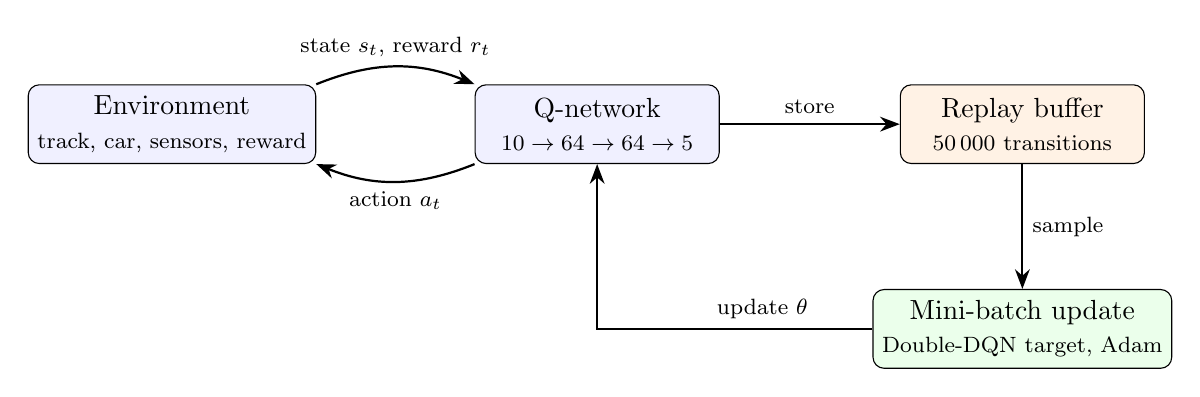
\begin{tikzpicture}[
  box/.style={draw,rounded corners,minimum width=3.1cm,minimum height=1.0cm,align=center,fill=blue!6},
  arr/.style={-{Stealth[length=2.5mm]},thick}]
  \node[box] (env) at (0,0) {Environment\\{\footnotesize track, car, sensors, reward}};
  \node[box] (agent) at (5.4,0) {Q-network\\{\footnotesize \(10\to64\to64\to5\)}};
  \node[box,fill=orange!10] (buf) at (10.8,0) {Replay buffer\\{\footnotesize 50\,000 transitions}};
  \node[box,fill=green!8] (opt) at (10.8,-2.6) {Mini-batch update\\{\footnotesize Double-DQN target, Adam}};
  \draw[arr] (env.north east) to[bend left=22] node[above,font=\footnotesize]{state \(s_t\), reward \(r_t\)} (agent.north west);
  \draw[arr] (agent.south west) to[bend left=22] node[below,font=\footnotesize]{action \(a_t\)} (env.south east);
  \draw[arr] (agent) -- node[above,font=\footnotesize]{store} (buf);
  \draw[arr] (buf) -- node[right,font=\footnotesize]{sample} (opt);
  \draw[arr] (opt.west) -| node[above,font=\footnotesize,pos=.2]{update \(\theta\)} (agent.south);
\end{tikzpicture}
\caption{The learning loop. The environment and the Q-network exchange states, rewards and actions; every transition is stored in the replay buffer, and mini-batches sampled from it are used to update the parameters \(\theta\) of the Q-network that chooses the actions.}
\label{fig:loop}
\end{figure}

\subsection{Track generation}
Each track is a closed loop whose centre line is a radial Fourier curve
\begin{equation}
  r(\phi)=R_0+\sum_{k=2}^{4}\frac{W}{k}\,u_k\cos(k\phi+\varphi_k),\qquad \phi\in[0,2\pi),
\end{equation}
with \(R_0=250\), \(W=70\), and random \(u_k\sim\mathcal U(0,1)\), \(\varphi_k\sim\mathcal U(0,2\pi)\) drawn from a seed.
The centre line is sampled at \(n=360\) points.
The signed curvature
\(\kappa=(x'y''-y'x'')/(x'^2+y'^2)^{3/2}\) is computed numerically, and a candidate curve is rejected unless its tightest bend has radius at least \(2.3\,h\), where \(h=32\) is the road half-width.
This guarantees that every generated track is physically drivable.
Walls are the centre line offset by \(\pm h\) along the unit normals, giving \(2n\) wall segments.
A different seed gives a different track, which we use to test generalisation.

\subsection{Vehicle model}
The car has position \((x,y)\), heading \(\theta\) and speed \(v\in[v_{\min},v_{\max}]=[1,5]\) (units per step).
There are five discrete actions:
\emph{coast}, \emph{steer left} (\(\theta\mathrel{+}=0.07\) rad), \emph{steer right} (\(\theta\mathrel{-}=0.07\) rad), \emph{accelerate} (\(v\mathrel{+}=0.15\)) and \emph{brake} (\(v\mathrel{-}=0.30\)).
After applying the action the car moves by
\begin{equation}
  x\leftarrow x+v\cos\theta,\qquad y\leftarrow y+v\sin\theta .
\end{equation}
The steering rate is independent of speed, a deliberate simplification that keeps the dynamics easy to reason about.
The car crashes (and the episode ends) when its distance to the nearest centre-line point exceeds \(h-r_c\), with car radius \(r_c=6\).
Progress is measured by the signed number of centre-line points the car has advanced, tracked with a windowed nearest-point search (so a car cannot ``teleport'' across to a distant part of the loop).

\subsection{Sensors}
The car is equipped with nine range sensors spread uniformly over a \(180^\circ\) fan centred on the heading (Figure~\ref{fig:sensors}).
Sensor \(j\) casts a ray with direction \(\mathbf d_j=(\cos(\theta+\alpha_j),\sin(\theta+\alpha_j))\) from the car position \(\mathbf o\) and has maximum range \(L=120\).
Against a wall segment starting at \(\mathbf p\) with edge vector \(\mathbf e\), the hit distance \(t\) and segment parameter \(u\) satisfy \(\mathbf o+t\mathbf d=\mathbf p+u\mathbf e\), which gives
\begin{equation}
  t=\frac{(\mathbf p-\mathbf o)\times\mathbf e}{\mathbf d\times\mathbf e},\qquad
  u=\frac{(\mathbf p-\mathbf o)\times\mathbf d}{\mathbf d\times\mathbf e},\qquad
  \mathbf a\times\mathbf b=a_xb_y-a_yb_x ,
\end{equation}
and a hit is valid when \(t\ge0\) and \(0\le u\le1\).
The distance returned by sensor \(j\) is the minimum valid \(t\), or \(L\) if nothing is hit.
The computation is fully vectorised over all rays and over the 202 wall segments nearest to the car, which makes it fast enough for thousands of simulation steps per second in pure NumPy.

\begin{figure}[H]
\centering
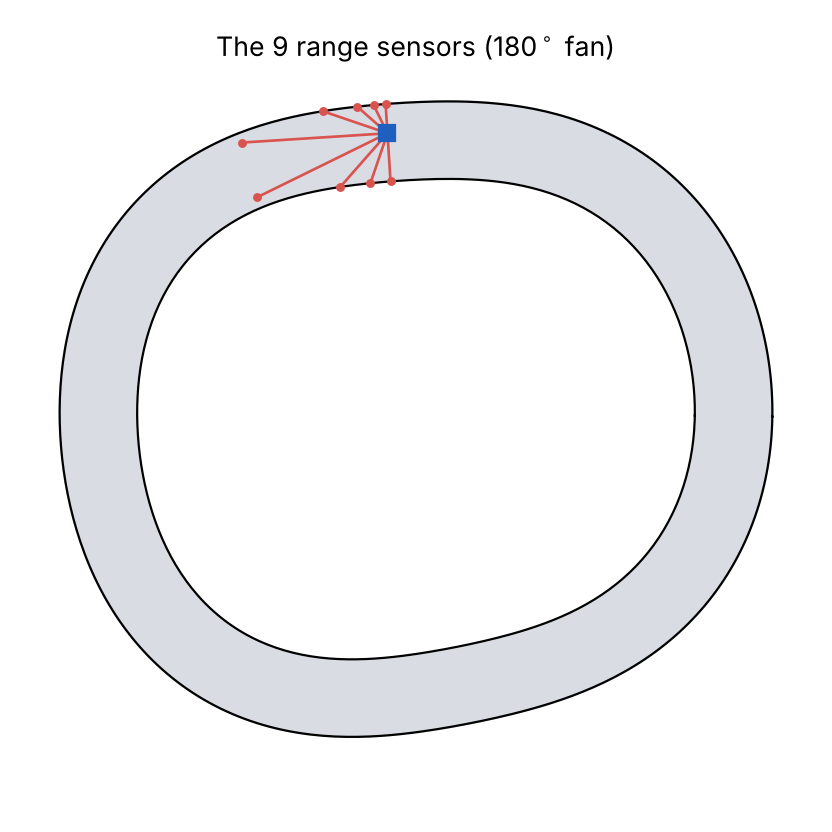
\includegraphics[width=0.52\linewidth]{figures/sensors.png}
\caption{The nine range sensors of the car (blue square) on a generated track. Each ray reports the distance to the nearest wall, capped at 120 units.}
\label{fig:sensors}
\end{figure}

\subsection{Observation and reward}
The observation is a 10-dimensional vector in \([0,1]^{10}\): the nine ray distances divided by \(L\), and the speed divided by \(v_{\max}\).
The agent does not receive its position, the map, or the road direction; it must infer everything from the sensors.

The reward at each step is
\begin{equation}
  r=\frac{v}{v_{\max}}\cos(\theta-\theta_{\text{road}})-\tfrac12\,p^{2},\qquad
  p=\max\!\left(0,\frac{0.25-\min_j \hat d_j}{0.25}\right),
\end{equation}
where \(\theta_{\text{road}}\) is the direction of the road at the car's position and \(\hat d_j\) are the normalised ray distances.
The first term rewards fast driving \emph{along} the road; the second is a mild penalty when any sensor sees a wall closer than a quarter of its range, which encourages staying away from the walls.
A crash gives \(r=-1\) and ends the episode.
Episodes also end after a fixed step limit (2000 in training); such time-limit endings are \emph{not} treated as terminal in the Bellman target, since the car is not actually in a terminal state.

\subsection{Neural network and back-propagation}
The Q-network is a multilayer perceptron \(10\to64\to64\to5\) with ReLU hidden units and a linear output (5\,189 parameters).
Weights use He initialisation \cite{he2015}.
For a mini-batch \(X\) the forward pass is \(h_0=X\), \(h_{i}=\operatorname{ReLU}(h_{i-1}W_i+b_i)\) for hidden layers, and a linear last layer.
Given \(\partial\ell/\partial h_L\) (non-zero only for the action that was taken), the backward pass is
\begin{equation}
  \frac{\partial\ell}{\partial W_i}=h_{i-1}^{\!\top}\,\Delta_i,\qquad
  \frac{\partial\ell}{\partial b_i}=\sum_{\text{batch}}\Delta_i,\qquad
  \Delta_{i-1}=(\Delta_iW_i^{\!\top})\odot\mathbb 1[h_{i-1}>0].
\end{equation}
Parameters are updated with Adam \cite{kingma2015} (\(\beta_1=0.9\), \(\beta_2=0.999\)) with global gradient-norm clipping at 10.

\paragraph{Gradient check.}
As in the micrograd tradition, the hand-written gradients are verified against centred finite differences, \((\mathcal L(w+\epsilon)-\mathcal L(w-\epsilon))/2\epsilon\) with \(\epsilon=10^{-6}\), on a random \(6\to8\to7\to4\) network.
The worst relative error over all weights and biases is \(3.1\times10^{-7}\), well below the \(10^{-5}\) threshold, so the back-propagation is correct.

\subsection{The DQN training algorithm}
\begin{enumerate}[label=\textbf{\arabic*.}]
  \item Initialise the online network \(Q_\theta\) and copy it to the target network \(Q_{\theta^-}\); empty the replay buffer.
  \item At each environment step, choose a random action with probability \(\varepsilon\) (decayed linearly from 1.0 to 0.05 over 25\,000 steps), otherwise \(a=\arg\max_aQ_\theta(s,a)\).
  \item Execute \(a\), observe \(r\), \(s'\) and the crash flag \(d\); store \((s,a,r,s',d)\) in the replay buffer.
  \item After a warm-up of 1\,000 steps, every second step sample a mini-batch of 64 transitions, compute the targets by Eq.~\eqref{eq:target}, take one Adam step on the Huber loss.
  \item Every 500 updates copy \(\theta\) into \(\theta^-\).
  \item When an episode ends (crash or step limit), reset the car to a random point on the track with a random lateral offset, heading noise and speed.
\end{enumerate}
Random start positions matter: without them the agent would only ever practise the first corner of the track.

\begin{table}[H]
\centering
\caption{Hyper-parameters used in all experiments (no tuning was performed).}
{\small\setlength{\tabcolsep}{4pt}
\begin{tabular}{@{}ll@{\qquad}ll@{}}
\toprule
\multicolumn{2}{c}{\textbf{Learning}} & \multicolumn{2}{c}{\textbf{Environment}}\\
\midrule
Discount \(\gamma\) & 0.97 & Road half-width \(h\) & 32 \\
Learning rate (Adam) & \(10^{-3}\) & Sensor range \(L\) / count & 120 / 9 \\
Batch size & 64 & Speed range \([v_{\min},v_{\max}]\) & [1, 5] \\
Replay capacity & 50\,000 & Steering per step & 0.07 rad \\
Target sync & every 500 updates & Acceleration / braking & +0.15 / \(-0.30\) \\
Update frequency & every 2 steps & Car radius \(r_c\) & 6 \\
Warm-up & 1\,000 steps & Episode limit (train / eval) & 2\,000 / 3\,000 \\
\(\varepsilon\) schedule & \(1\to0.05\) in 25\,000 steps & Hidden layers & \(64,64\) (ReLU) \\
\bottomrule
\end{tabular}}
\end{table}

%=====================================================================
\section{Software and User Interface}
%=====================================================================
All code is in a single file, \code{self\_driving\_car.py}, written in Python with NumPy; the interface uses Tkinter, which is part of the standard Python distribution.
The file is organised in clearly separated components:

\begin{center}
\begin{tabular}{@{}ll@{}}
\toprule
\textbf{Component} & \textbf{Responsibility}\\
\midrule
\code{Track}    & track generation, wall geometry, nearest-point search\\
\code{CarEnv}   & vehicle dynamics, ray casting, reward, \code{reset()/step()} interface\\
\code{MLP}      & network forward/backward pass, Adam, save/load, gradient check\\
\code{DQNAgent} & replay buffer, Double-DQN update, target network\\
\code{Trainer}  & exploration schedule, episode bookkeeping and history\\
\code{App}      & Tkinter interface\\
CLI             & \code{gui}, \code{train}, \code{eval}, \code{gradcheck} commands\\
\bottomrule
\end{tabular}
\end{center}

\paragraph{The interface.}
Running \code{python self\_driving\_car.py} opens a window with the track on the left and a control panel on the right.
The car and its nine sensor rays are drawn live (green/yellow/red according to how close the wall is).
The panel offers:
\begin{itemize}
  \item \textbf{Start/Pause} training (also bound to the space bar) and a slider for the number of simulation steps per displayed frame (1--400), so learning can be watched in slow motion or fast-forwarded;
  \item \textbf{Reset car}, \textbf{New random track} (the agent keeps its knowledge, which demonstrates generalisation live), and \textbf{Reset agent};
  \item \textbf{Drive manually}: the user takes over with the arrow keys, which is useful to appreciate how difficult the task is;
  \item \textbf{Greedy} mode (no random exploration), \textbf{Show sensors} toggle, and \textbf{Save/Load model};
  \item live statistics (steps, episodes, \(\varepsilon\), average distance, return and crash rate over the last 50 episodes, TD loss) and a small learning curve.
\end{itemize}
The quantitative results in this report were produced with the headless commands (\code{train}, \code{eval}), which use exactly the same \code{Trainer} and environment code as the interface.

%=====================================================================
\section{Experiments}
%=====================================================================
\subsection{Protocol}
The agent is trained for 150\,000 environment steps on a single track (seed~1) and is then evaluated with the greedy policy (\(\varepsilon=0\)).
Each evaluation consists of 20 episodes of up to 3\,000 steps, starting at random points on the track.
We evaluate on the training track and on four unseen tracks (seeds 2--5) generated by the same procedure.
Three policies are compared:
\begin{description}[leftmargin=1.5em]
  \item[Random:] uniformly random actions.
  \item[Heuristic:] a hand-written controller that steers toward the side with more free space, brakes if something is straight ahead, and otherwise accelerates up to about 80\,\% of the top speed.
  \item[DQN:] the trained agent.
\end{description}
We report (i) \emph{mean laps}: the distance travelled along the track before crashing or reaching the 3\,000-step limit, expressed in laps; (ii) the \emph{survival rate}: the fraction of episodes that did not end in a crash; and (iii) the mean speed.
The whole training procedure was repeated with three random seeds (0, 1, 2), which change the network initialisation, exploration and start-position randomness, but not the training track.

\subsection{Learning behaviour}
Figure~\ref{fig:learning} shows the learning curve of seed~0.
For the first roughly 10\,000 steps the car crashes after a short distance.
Between about 10\,000 and 17\,000 steps, the performance jumps: the first episode that lasts the full 2\,000 steps without crashing occurs at step 17\,931 (seed~0), 17\,036 (seed~1) and 16\,909 (seed~2), i.e.\ \((1.73\pm0.05)\times10^{4}\) steps; this happens while \(\varepsilon\) is still above 0.3, i.e.\ the car already survives 2\,000 steps even though roughly a third of its actions are random.
Because episodes become much longer once the car survives, only 167--192 episodes are completed in the whole run, of which 101--126 ended in a crash. Of the 195 episodes that ended after step 20\,000 (65 per seed), only 2 were crashes (one in seed~0 and one in seed~1).
The curve is nearly flat afterwards, with one visible dip near step 81\,000 (seed~0) where a single episode ended early with a crash; this is a typical sign of the residual instability of value-based deep RL, and the policy recovered immediately.

\begin{figure}[H]
\centering
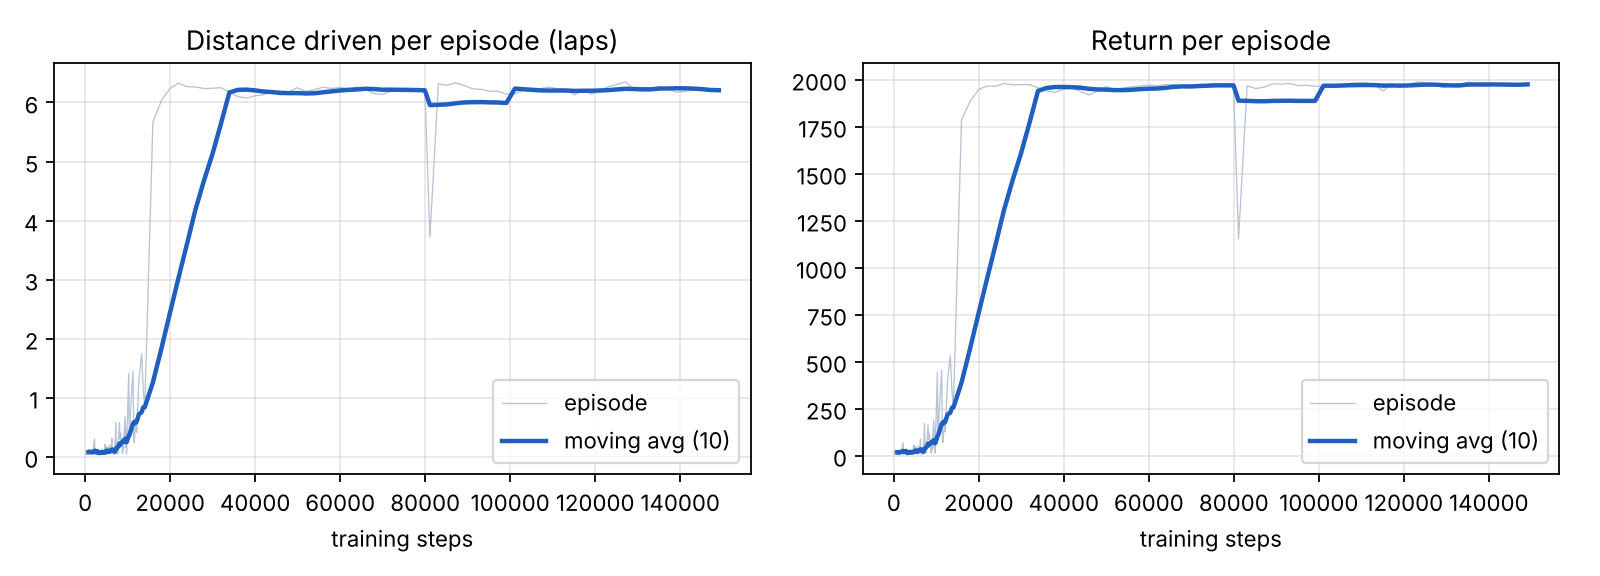
\includegraphics[width=\linewidth]{figures/learning_curve.png}
\caption{Learning curve (seed 0). The light line shows individual episodes, each plotted at the training step where it ended; the thick line is a 10-episode moving average. Episodes are capped at 2\,000 steps, so distance saturates near 6.3 laps.}
\label{fig:learning}
\end{figure}

\subsection{Quantitative results}
Table~\ref{tab:tracks} gives the per-track results for seed~0 and Table~\ref{tab:seeds} summarises the three seeds.

\begin{table}[H]
\centering
\caption{Mean laps over 20 evaluation episodes (3\,000-step limit) per track, for the seed-0 agent. Survival rate was 0.00 for the random driver and 1.00 for both the heuristic and the DQN on every track.}
\label{tab:tracks}
\begin{tabular}{@{}lcccc@{}}
\toprule
\textbf{Track} & \textbf{Random} & \textbf{Heuristic} & \textbf{DQN} & \textbf{DQN std.\ dev.}\\
\midrule
Training track (seed 1) & 0.08 & 7.88 & 9.19 & 0.01\\
Unseen track (seed 2)   & 0.08 & 7.79 & 9.06 & 0.01\\
Unseen track (seed 3)   & 0.08 & 7.84 & 9.14 & 0.01\\
Unseen track (seed 4)   & 0.08 & 7.63 & 8.89 & 0.01\\
Unseen track (seed 5)   & 0.09 & 7.80 & 9.10 & 0.01\\
\bottomrule
\end{tabular}
\end{table}

\begin{table}[H]
\centering
\caption{Results for three independent training runs. ``Unseen'' is the average over the four unseen tracks. Survival of the DQN was 1.00 in every case.}
\label{tab:seeds}
\begin{tabular}{@{}lcccc@{}}
\toprule
\textbf{Seed} & \textbf{First crash-free} & \textbf{DQN laps,} & \textbf{DQN laps,} & \textbf{Training}\\
              & \textbf{full episode (step)} & \textbf{training track} & \textbf{unseen (mean)} & \textbf{time (s)}\\
\midrule
0 & 17\,931 & 9.19 & 9.05 & 54\\
1 & 17\,036 & 9.48 & 9.36 & 57\\
2 & 16\,909 & 9.30 & 9.20 & 56\\
\midrule
\textbf{Mean \(\pm\) std} & \(17\,292\pm455\) & \(9.32\pm0.12\) & \(9.20\pm0.13\) & 56\\
\bottomrule
\end{tabular}

\smallskip
{\footnotesize For reference (identical for every seed, since they are deterministic): heuristic 7.76 laps on the unseen tracks, random driver 0.08 laps.}
\end{table}

\begin{figure}[H]
\centering
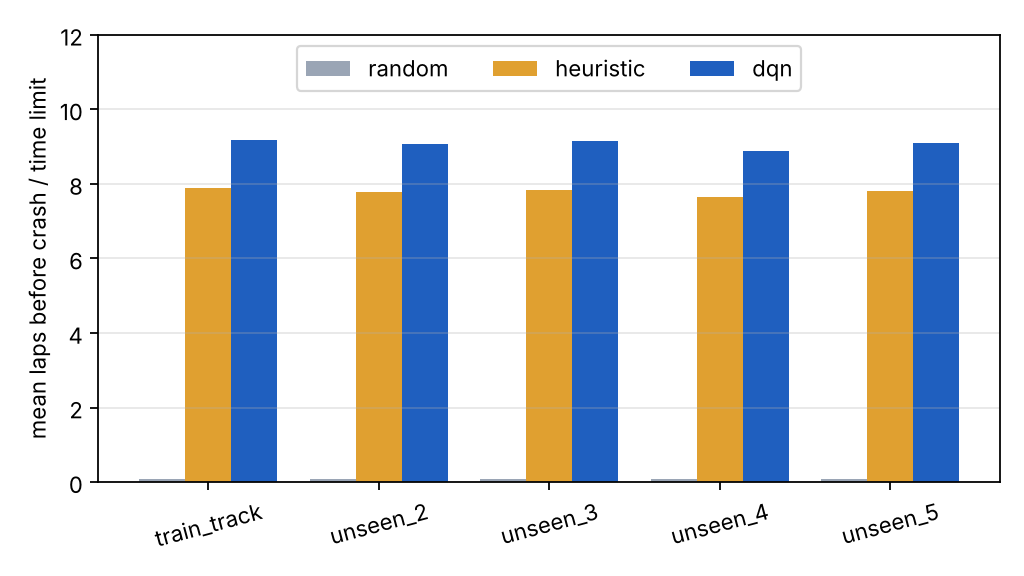
\includegraphics[width=0.78\linewidth]{figures/comparison.png}
\caption{Mean laps for the three policies on the training track and four unseen tracks (seed-0 agent).}
\label{fig:comparison}
\end{figure}

\begin{figure}[H]
\centering
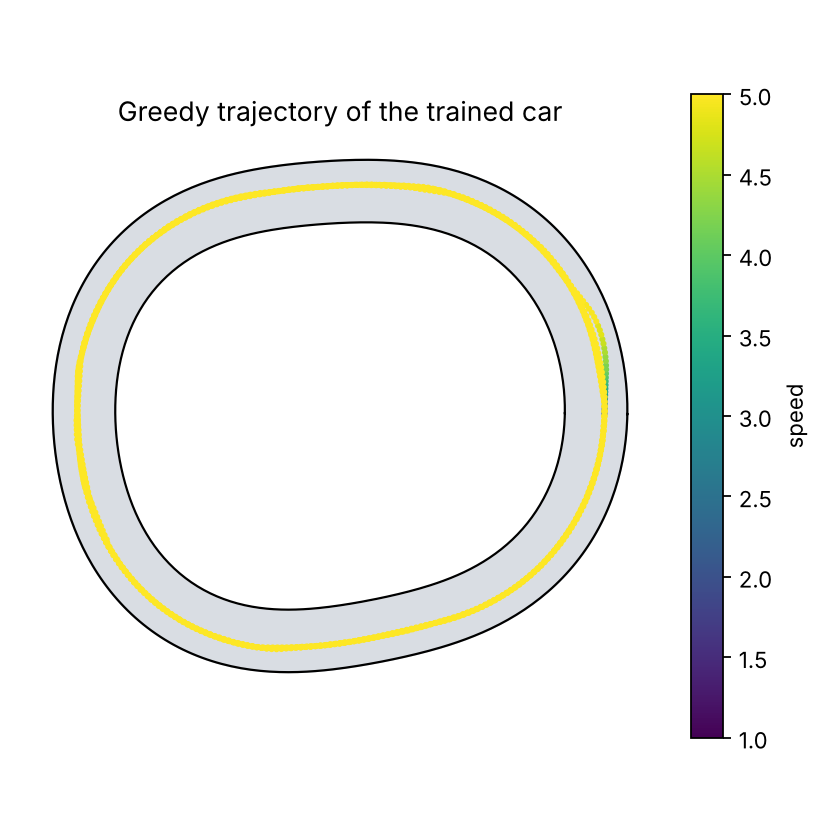
\includegraphics[width=0.52\linewidth]{figures/trajectory.png}
\caption{Greedy trajectory of the trained car on the training track, coloured by speed. After a short initial correction the car holds the maximum speed (5) and follows the middle of the road.}
\label{fig:trajectory}
\end{figure}

\subsection{Interpretation}
\begin{itemize}
  \item \textbf{Learning works.} The random driver covers 0.08 laps before crashing; the trained agent never crashed in any of the \(5\times20\) evaluation episodes per seed, i.e.\ it safely drove for 3\,000 steps each time.
  \item \textbf{Why the DQN scores more laps than the heuristic.} Both controllers survive every episode, so the lap count is mainly a measure of \emph{speed}. The DQN drives at an average speed of 4.99 (essentially the top speed 5), whereas the heuristic averages 4.07. With a 3\,000-step limit and a track length of about 1\,583 units, the theoretical maximum is \(3000\times5/1583\approx9.5\) laps, and the DQN reaches 8.9--9.5 across all seeds and tracks. The comparison should therefore be read as ``the learned agent drives as fast as physically allowed without crashing, while the simple controller is cautious'', not as evidence that the DQN is a better steerer in general. The heuristic is a deliberately simple baseline and was not tuned for speed.
  \item \textbf{Generalisation.} Without any retraining, the agent drove all four unseen tracks without a crash and with almost the same distance as on the training track (Table~\ref{tab:seeds}). This is plausible because the observation consists only of \emph{relative} quantities (distances to walls and speed), so a good policy for one bend is also a good policy for similar bends elsewhere.
  \item \textbf{Cost.} Training took about 56 seconds on one CPU core (about 2\,700 steps/s including the gradient updates), which is why a pure-NumPy implementation is perfectly adequate for this problem.
\end{itemize}

%=====================================================================
\section{Limitations and Honest Caveats}
%=====================================================================
\begin{itemize}
  \item \textbf{Same family of tracks.} The unseen tracks come from the same random generator as the training track (smooth loops of similar width and curvature). Success on them does not imply that the agent could handle sharp hairpins, intersections, or narrower roads.
  \item \textbf{Saturated metric.} Because both good controllers survive the whole evaluation, the lap metric is capped by the speed limit and the 3\,000-step window. A finer comparison would require lap times, harder tracks, or longer horizons.
  \item \textbf{Simplified world.} The vehicle model has no tyre slip, inertia or speed-dependent steering, and there is no other traffic. The state is only the current sensor reading plus speed (no memory), so the agent cannot, for example, anticipate a bend it cannot yet see.
  \item \textbf{No hyper-parameter search; few seeds.} A single hyper-parameter setting was used and only three seeds were run. The results are consistent across these seeds, but three seeds are not enough for strong statistical claims, and the small standard deviations in Table~\ref{tab:seeds} should be read in that light. The single dip in Figure~\ref{fig:learning} shows that training is not perfectly stable.
  \item \textbf{Interface vs.\ experiments.} The graphical interface is a thin layer over the same trainer and environment classes, but the numbers in this report were produced with the headless commands, not through the window.
\end{itemize}

%=====================================================================
\section{Conclusion and Future Work}
%=====================================================================
We implemented, from scratch and in plain Python/NumPy, a complete self-driving-car learning system: a procedurally generated track, a sensor-equipped car, a hand-written neural network with verified gradients, a Double-DQN agent, and an interactive interface.
The agent learns to drive crash-free at maximum speed in roughly 17\,000 steps (under ten seconds of CPU time; the full 150\,000-step run takes under a minute) and transfers to unseen tracks of the same kind without retraining.

Natural extensions are: (i) pixel observations with a convolutional network, as in the original ConvNetJS demonstrations; (ii) other cars and traffic, which makes collision avoidance and overtaking part of the task; (iii) continuous steering and throttle with an actor--critic method; (iv) more demanding track families (hairpins, varying width) and a curriculum; (v) a recurrent or frame-stacked state so the agent has memory; and (vi) prioritised replay or n-step returns to speed up learning further.

%=====================================================================
\section*{How to Reproduce}
%=====================================================================
\begin{verbatim}
pip install numpy matplotlib          # matplotlib is optional (figures)
python self_driving_car.py gradcheck  # verify back-propagation
python self_driving_car.py            # open the interactive window
python self_driving_car.py train --steps 150000 --out runs/run1 --seed 0
python self_driving_car.py eval --model runs/run1/model.npz
\end{verbatim}
The \code{train} command writes the model, the learning history, a JSON file of evaluation results and the figures used in this report (\code{learning\_curve}, \code{trajectory}, \code{sensors}, \code{comparison}) into the output folder.
Seeds 1 and 2 correspond to \code{--seed 1} and \code{--seed 2}.
Absolute timings depend on the machine; the numerical results depend on the NumPy version only through floating-point details.

%=====================================================================
\begin{thebibliography}{99}
\bibitem{karpathy-rldemo} A.~Karpathy. \emph{ConvNetJS: Deep Q Learning demo} (browser-based self-driving car with distance sensors). \url{https://cs.stanford.edu/people/karpathy/convnetjs/demo/rldemo.html}.
\bibitem{karpathy-micrograd} A.~Karpathy. \emph{micrograd}: a tiny scalar-valued autograd engine. \url{https://github.com/karpathy/micrograd}.
\bibitem{karpathy-hackers} A.~Karpathy. \emph{Hacker's guide to Neural Networks}. \url{https://karpathy.github.io/neuralnets/}.
\bibitem{sutton-barto} R.~S. Sutton and A.~G. Barto. \emph{Reinforcement Learning: An Introduction}, 2nd ed. MIT Press, 2018.
\bibitem{watkins-dayan} C.~J.~C.~H. Watkins and P.~Dayan. Q-learning. \emph{Machine Learning}, 8:279--292, 1992.
\bibitem{lin1992} L.-J. Lin. Self-improving reactive agents based on reinforcement learning, planning and teaching. \emph{Machine Learning}, 8:293--321, 1992.
\bibitem{mnih2015} V.~Mnih et al. Human-level control through deep reinforcement learning. \emph{Nature}, 518:529--533, 2015.
\bibitem{vanhasselt2016} H.~van Hasselt, A.~Guez and D.~Silver. Deep reinforcement learning with double Q-learning. In \emph{AAAI}, 2016.
\bibitem{huber1964} P.~J. Huber. Robust estimation of a location parameter. \emph{Annals of Mathematical Statistics}, 35(1):73--101, 1964.
\bibitem{he2015} K.~He, X.~Zhang, S.~Ren and J.~Sun. Delving deep into rectifiers: surpassing human-level performance on ImageNet classification. In \emph{ICCV}, 2015.
\bibitem{kingma2015} D.~P. Kingma and J.~Ba. Adam: a method for stochastic optimization. In \emph{ICLR}, 2015.
\end{thebibliography}

%=====================================================================
\appendix
\section{Complete Source Code}\label{app:code}
The listing below is the complete file \code{self\_driving\_car.py}.
\lstinputlisting{self_driving_car.py}

\end{document}
